\documentclass[border=6pt]{standalone}
\usepackage{tikz}
\usetikzlibrary{arrows.meta,positioning}
\begin{document}
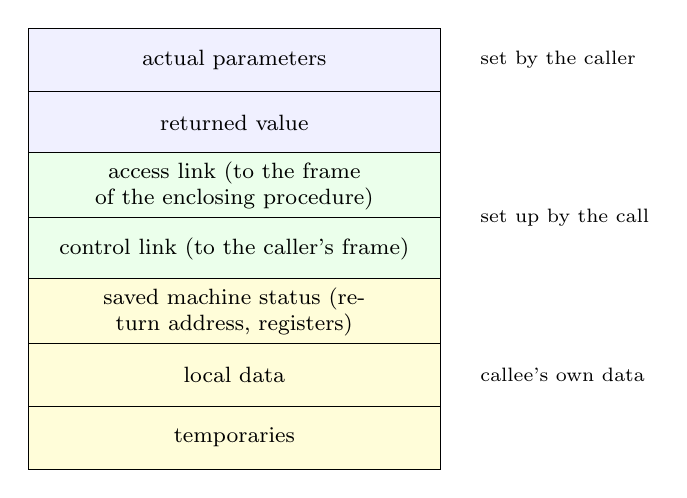
\begin{tikzpicture}[>=Stealth,font=\small,
  cell/.style={draw,minimum width=5.2cm,text width=5.0cm,minimum height=0.8cm,align=center,font=\footnotesize}]
\node[cell,fill=blue!6]  (c1) at (0,0)    {actual parameters};
\node[cell,fill=blue!6]  (c2) at (0,-0.8) {returned value};
\node[cell,fill=green!8] (c3) at (0,-1.6) {access link (to the frame of the enclosing procedure)};
\node[cell,fill=green!8] (c4) at (0,-2.4) {control link (to the caller's frame)};
\node[cell,fill=yellow!15] (c5) at (0,-3.2) {saved machine status (return address, registers)};
\node[cell,fill=yellow!15] (c6) at (0,-4.0) {local data};
\node[cell,fill=yellow!15] (c7) at (0,-4.8) {temporaries};
\node[font=\scriptsize,anchor=west] at (3.0,0) {set by the caller};
\node[font=\scriptsize,anchor=west] at (3.0,-2.0) {set up by the call};
\node[font=\scriptsize,anchor=west] at (3.0,-4.0) {callee's own data};
\end{tikzpicture}
\end{document}
